% Block diagram of Witsenhausen's counterexample.
% Compile to web/figures/problem.svg with:  python scripts/build_figures.py
\documentclass[tikz,border=4pt]{standalone}
\usepackage{amsmath,amssymb}
\usetikzlibrary{arrows.meta,positioning,calc}
\begin{document}
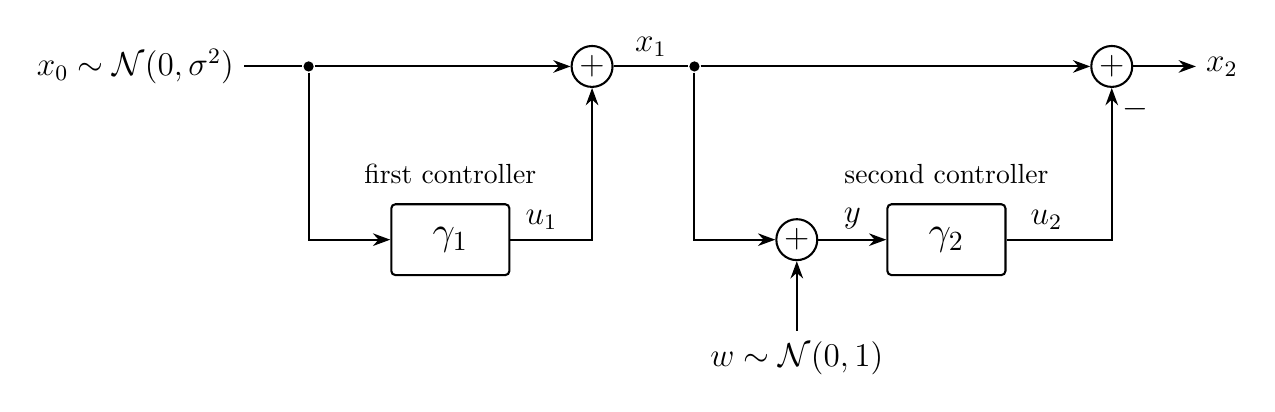
\begin{tikzpicture}[
    >={Stealth[length=2.2mm,width=1.6mm]},
    line width=0.75pt,
    font=\large,
    ctrl/.style={draw, rounded corners=1.5pt, minimum width=15mm, minimum height=9mm, align=center, font=\Large},
    sum/.style={draw, circle, inner sep=0pt, minimum size=5.2mm},
    dot/.style={circle, fill, inner sep=0pt, minimum size=1.3mm},
    ctrlname/.style={font=\normalsize},
  ]
  % plant path (top row)
  \node (x0)  at (0,0)      {$x_0 \sim \mathcal{N}(0,\sigma^2)$};
  \node[dot]  (b1) at (2.2,0)  {};
  \node[sum]  (s1) at (5.8,0)  {$+$};
  \node[dot]  (b2) at (7.1,0)  {};
  \node[sum]  (s3) at (12.4,0) {$+$};
  \node (x2)  at (13.8,0)   {$x_2$};

  % controllers (bottom row)
  \node[ctrl] (c1) at (4.0,-2.2)  {$\gamma_1$};
  \node[sum]  (s2) at (8.4,-2.2)  {$+$};
  \node[ctrl] (c2) at (10.3,-2.2) {$\gamma_2$};
  \node (w) at (8.4,-3.7) {$w \sim \mathcal{N}(0,1)$};

  % signal flow
  \draw     (x0) -- (b1);
  \draw[->] (b1) -- (s1);
  \draw[->] (b1) |- (c1);
  \draw[->] (c1) -| node[pos=0.19, above] {$u_1$} (s1);
  \draw     (s1) -- node[above] {$x_1$} (b2);
  \draw[->] (b2) -- (s3);
  \draw[->] (b2) |- (s2);
  \draw[->] (w)  -- (s2);
  \draw[->] (s2) -- node[above] {$y$} (c2);
  \draw[->] (c2) -| node[pos=0.19, above] {$u_2$} node[pos=0.93, right] {$-$} (s3);
  \draw[->] (s3) -- (x2);

  % names of the two controllers; what each one sees and pays is in the caption
  \node[ctrlname, above=1.2mm of c1] {first controller};
  \node[ctrlname, above=1.2mm of c2] {second controller};
\end{tikzpicture}
\end{document}
